\subsection{NVD Case Study}
\label{sec:evaluation_nvd}
The U.S. National Institute of Standards and Technology (NIST) maintains the National Vulnerability Database (NVD) ~\footnote{https://nvd.nist.gov/}, an online database of publicly reported software vulnerabilities, with over 79,000 vulnerabilities dating back to 1988. Vulnerability reporters assign each vulnerability a Common Vulnerability Scoring System (CVSS) score and associated CVSS base metrics, according to the scheme defined in the CVSS guide~\cite{mell2007complete}.  

\subsubsection{Data selection}
\label{sec:evaluation_nvd_selection}
 We translate the CVSS metrics into the terms of our model constructs and measurements. For each structural model construct, we present our metric associations and the rationale behind them.
 
\textbf{Asset Value}
The CVSS Confidentiality Impact, Integrity Impact, and Availability Impact metrics measure the degree of loss of confidentiality, integrity, and availability represented by a reported vulnerability~\cite{mell2007complete}. The CVSS Impact values:
	\begin{itemize}
		\item 'None' indicates no impact, 
		\item 'Partial' indicates partial impact, and 
		\item 'Complete' indicates 'Complete' impact to the CIA property of the system by the exploited vulnerability.  
	\end{itemize}
We model each Impact metric as a component of Asset Value, theorizing that confidentiality, integrity, and availability impacts change based on the usage context in which the software is run, e.g. the value of the assets managed. We translate None/Partial/Complete to an ordinal scale to model increasing CIA impact risk.

\textbf{Software Risk}
\label{sec:evaluation_nvd_selection_risk}
The CVSS Access Vector, Access Complexity, and Authentication metrics capture how a vulnerability is accessed and whether or not extra conditions are required to exploit it.~\cite{mell2007complete}. We translate these metrics into the terms of our model constructs and measurements. For each metric, we now quote the CVSS guide definition, and give a rationale for the associations we have defined:
\begin{itemize}
	\item Access Vector - measures how the vulnerability is exploited, in terms of network distance. Values:
	\begin{itemize}
		\item 'Local' requires the attacker to have physical access or an account on the system, \item 'Adjacent Network' requires access to the physical network on which the vulnerable software resides, and \item 'Network' requires only logical network acccess, e.g. remote access. 
	\end{itemize}
	We model Access Vector Risk as a component of Software Risk, theorizing that the vector value changes based on design choices made by the software development team. We translate the CVSS Access Vector values to an ordinal scale to model increasing `Access Vector Risk'.
	\item Access Complexity - measures the complexity of attack required to exploit a vulnerability once an attacker has gained access. Values: 
	\begin{itemize}
		\item 'High' indicates specialized/elevated access is required to exploit the vulnerability, 
		\item 'Medium' indicates that some access is required to exploit the vulnerability, and \item 'Low' indicates that the vulnerability can be exploited with default/no special access.  
	\end{itemize}
	We model Access Complexity Risk as a component of Software Risk, theorizing that the complexity value changes based on design choices made by the software development team. We translate the CVSS Access Complexity  to an ordinal scale to model increasing `Access Complexity Risk'.
	\item Authentication - measures the number of times an attacker must authenticate to exploit a vulnerability. Values: 
	\begin{itemize}
		\item 'Multiple' indicates an attacker must authenticate two or more times to exploit the vulnerability, 
		\item 'Single' indicates that an attacker must authenticate once to exploit the vulnerability, and 
		\item 'None' indicates that the vulnerability can be exploited without authenticating.  
	\end{itemize}
	We model Authentication as a component of Software Risk, theorizing that the authentication requirement changes based on design choices made by the software development team. We translate CVSS Authentication values to an ordinal scale to model increasing `Authentication Risk'.
\end{itemize}
  
\textbf{Adherence}
We model Adherence via the passage of time; we take the year each vulnerability is reported as indicative of the state of security practice adherence at the time the vulnerability was reported. We define an `adherence' metric for each vulnerability as the difference, in years, between the vulnerability's publication date and the initial year in the NVD database. If software quality (presumed to be caused by practice adherence) is increasing, we would expect to see a positive correlation between year and the CVSS impact metrics.  In an earlier test of this hypothesis, Kaminsky et al. ~\cite{kaminsky2011showing} fuzzed ten years of office software releases, confirming that software quality had improved over the previous decade, as measured by crash counts per software release over time. 
    
\textbf{Outcomes}
We obtain a metric for Outcomes by counting per-project, per-year vulnerabilities. We treat each unique software name in the NVD records as a distinct project, and sum all vulnerabilities for a project, reflecting our theorized post-release vulnerability count metric. We group each project by its (software) name, and by publication year, taking the mean of the remaining CVSS metrics to represent that project/publication year. 
% plot vuln count over time
% plot cvss score average
% plot three impact metrics
% plot three access metrics	

\textbf{NVD Data Examples}
To illustrate how data is prepared for use in SEM estimation, Table \ref{tab:nvd_data_examples} presents data from an example project, the Amazon flexible payments service, which experienced two vulnerabilities in 2012. The table presents the original data rows, the translated version of each row, and the project summary row, assembled from the translated rows, used in SEM estimation.

\begin{table}
	\begin{center}	
		\caption{NVD Original and Summarized Data for Example Project ()Amazon flexible\_payments\_service)}
		\label{tab:nvd_data_examples}
		\begin{scriptsize}
			\begin{tabular}{p{3cm}p{1.5cm}p{1cm}p{1.5cm}p{1cm}p{1cm}}
				&&&&&\\[-1.8ex]\hline 
				\hline &&&&\\[-1.8ex] 
				Field & Original & Translated & Original & Translated & Project Summary \\
				\hline &&&&&\\[-1.8ex] 				
				CVE Count &  1 & 1 & 1 & 1 & 2\\
				&&&&& 1.10\\
				Pub Year & 2012 & 2012 & 2012 & 2012 & 2012\\
				Adherence & & 5.26 & & 5.26 & 5.26 \\				
				CVSS Auth & NONE & 1 & NONE & 1 & 1 \\
				Access Vector & NETWORK & 3 & NETWORK & 3 & 3 \\
				Access Complexity & MEDIUM & 2 & MEDIUM & 2 & 2 \\
				Conf Impact & PARTIAL & 2 & PARTIAL & 2 & 2\\
				Integ Impact & PARTIAL & 2 & PARTIAL & 2 & 2\\
				Avail Impact & NONE & 1 & NONE & 1 & 1 \\
				\hline &&&&&\\[-1.8ex] 		
			\end{tabular}
		\end{scriptsize}
	\end{center}
\end{table}
			
			
\subsubsection{Data collection}
We collected the entire NVD dataset as of February 2017, but limit our analysis to complete years, from the year 2001 to 2016. The dataset includes vulnerabilities dating to 1988, but years previous to 2001 had relatively low activity (we measured activity for a year as the ratio of vulnerabilities reported that year to the average vulnerabilities per year over the NVD history. Activity first exceeded half of the overall average in 2001.) We show NVD Vulnerability counts per year in Figure ~\ref{fig:nvd_vulns_year}.

\begin{figure}
	\centering
	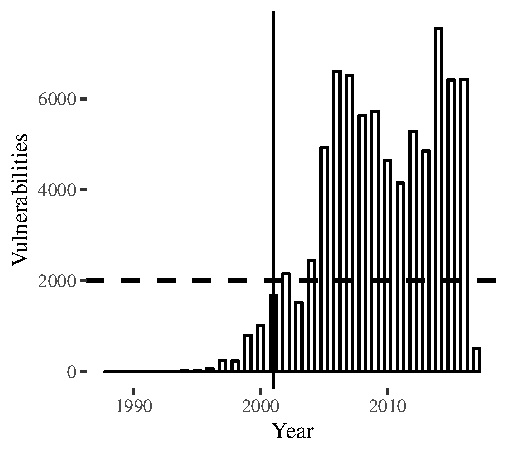
\includegraphics[width=.6\columnwidth]{nvd_vulns_year}
	\caption{NVD Vulnerability Count by Year}
	\label{fig:nvd_vulns_year}
\end{figure}
% stargazer(rtrunc)
% Table created by stargazer v.5.2 by Marek Hlavac, Harvard University. E-mail: hlavac at fas.harvard.edu
% Date and time: Sun, Feb 26, 2017 - 22:57:53
\begin{table}[!htbp] \centering 
	\caption{NVD Project Demographics} 
	\label{tab:nvd_demog} 
	\begin{small}
	\begin{tabular}{@{\extracolsep{5pt}}lccccc} 
		\\[-1.8ex]\hline 
		\hline \\[-1.8ex] 
		Statistic & \multicolumn{1}{c}{N} & \multicolumn{1}{c}{Mean} & \multicolumn{1}{c}{St. Dev.} & \multicolumn{1}{c}{Min} & \multicolumn{1}{c}{Max} \\ 
		\hline \\[-1.8ex] 
		CVECount & 10,622 & 4.311 & 5.241 & 2 & 49 \\ 
		logCVECount & 10,622 & 1.466 & 0.533 & 1.099 & 3.912 \\ 
		cvss\_score & 10,621 & 6.139 & 1.429 & 1.200 & 10.000 \\ 
		adherence & 10,621 & 4.678 & 1.007 & 0.225 & 6.532 \\ 
		cvss\_auth & 10,622 & 2.905 & 0.224 & 0.000 & 3.000 \\ 
		cvss\_access\_vector & 10,622 & 2.794 & 0.486 & 0.000 & 3.000 \\ 
		cvss\_access\_complexity & 10,622 & 2.577 & 0.409 & 0.000 & 3.000 \\ 
		cvss\_conf\_impact & 10,622 & 1.833 & 0.504 & 0.000 & 3.000 \\ 
		cvss\_integ\_impact & 10,622 & 1.902 & 0.467 & 0.000 & 3.000 \\ 
		cvss\_avail\_impact & 10,622 & 1.833 & 0.552 & 0.000 & 3.000 \\ 
		\hline \\[-1.8ex] 
	\end{tabular} 
		\end{small}
	
\end{table} 

\subsubsection{Estimation}

Combining the structural and measurement models we have defined with the CVSS data collected from the NVD database, we have the model definition, expressed in lavaan syntax: 

\begin{equation}
\begin{split}
	SoftwareRisk &=\sim cvss\_access\_vector \\ 
	&+ cvss\_access\_complexity + cvss\_auth\\
	AssetImpact &=\sim cvss\_conf\_impact\\
	&+ cvss\_integ\_impact + cvss\_avail\_impact\\
	Outcomes &=\sim logCVECount\\
	Adherence &=\sim adherence\\
	Outcomes &\sim SoftwareRisk + Adherence + AssetValue\\
	SoftwareRisk &\sim Adherence\\
\end{split}
\end{equation}		

\subsubsection{Model Fit} 
In terms of global fit, the fit index results for the initial NVD model were outside the range of standard fit criteria thresholds, as shown in the NVD column of Table \ref{tab:results_fit_all}, making the parameter estimates unreliable. 

\subsubsection{Re-specification}
The base adherence and CVE Count metrics had variances two magnitudes larger than the other variables. We scaled adherence, and took the log of CVE Count to bring them within range of the other variables. The variation among the 22,000+ projects with exactly one vulnerability caused numeric problems for the estimation algorithm, and we elected to treat the group as outliers and drop them from consideration. We, further, excluded projects with 50 or more vulnerabilities as outliers (79 projects). After the exclusions, 10621 projects remained in the analyzed dataset.

The re-specified model (post-rescaling and outlier exclusion) had global fit characteristics within the traditional fit criteria thresholds, as shown in the Respecified NVD column of Table \ref{tab:results_fit_all}. We present the parameter estimates for the Respecified NVD model in the results, and discuss the implications in Section \ref{sec:case_nvd_discussion}.

\subsubsection{Reporting Results}
\label{sec:case_nvd_results}

Table \ref{tab:results_fit_all} presents the fit measure results for the NVD  and Respecified NVD models (as well as for the other case study models). We report the estimated parameter values, unstandardized, for the Respecified NVD structural and measurement models in \ref{tab:results_nvd}. We present the standardized parameter estimates, and the residuals, in the context of the full structural and measurement models in Figure \ref{fig:nvd_model_respecified_estimates}.

\begin{table*}
	\begin{center}	
		\caption{Global Fit Measures and Results}
			\label{tab:results_fit_all}
			\begin{tabular}{p{3cm}p{1cm}|p{2cm}p{2cm}p{2cm}}
				\\[-1.8ex]\hline 
				\hline \\[-1.8ex] 
				Fit Measure & Threshold & NVD	& Respecified NVD & Respecified CII  \\
				\hline \\[-1.8ex] 				
				Number of observations &  & $10621$  & $10621$ & $343$  \\				
				Model chi-square &  & $2759.88$ & 1068.25 & $259$  \\				
				Model d.f. &  & $17$ & $18$ & $52$  \\		
				Model p-value & $\leq 0.01$ & $0.0$ & $0.0$ & $0.0$  \\
				RMSEA & $\leq 0.10$ &  $0.12$ &  $0.07$ & $0.108$   \\
				CFI & $> 0.90$ & $0.83$ & $0.93$  & $0.702$  \\
				SRMR & $< 0.08$ & $0.08$ & $0.06$ & $0.08$  \\
				\hline \\[-1.8ex] 				
			\end{tabular}
	\end{center}
\end{table*}

\begin{table}
	\begin{center}	
		\caption{NVD Respecified Model Results}
		\label{tab:results_nvd}
		\begin{tabular}{l|rrrr}
				\\[-1.8ex]\hline 
				\hline \\[-1.8ex] 
			\textit{Latent Variables}:  & & & & \\  
			$\sim$ Measured variables& Estimate & Std.Err & z$-$value & $P(>|z|)$ \\
				\hline \\[-1.8ex]
			$SoftwareRisk =\sim$  & & & & \\                                   
			cvss\_ccss\_vctr   & 1.000 & &  & \\                             
			cvss\_ccss\_cmpl &  $-$0.166 &   0.035 &  $-$4.86 &   0.000\\
			cvss\_auth     &   $-$1.498  &  0.164  & $-$9.125   & 0.000\\
			$AssetImpact =\sim$     & & & & \\                                    
			cvss\_conf\_mpct   & 1.000     & & & \\                       
			cvss\_intg\_mpct   & 0.797   & 0.011 & 70.746 &   0.000 \\
			cvss\_aval\_mpct  &  0.872   & 0.013 & 67.584   & 0.000 \\
			$Outcomes =\sim$    & & & & \\                                     
			logCVECount     &  1.000  & & & \\                          
			$Adherence =\sim$   & & & & \\                                      
			adherence    &     1.000        & & & \\                    
			Regressions:  & & & & \\  
			%& Estimate & Std.Err & z$-$value & $P(>|z|)$ \\
			$Outcomes \sim$         & & & & \\                                     
			SoftwareRisk   &  1.092 &   0.162 & 6.754 &   0.000 \\
			%Adherence       &  $-$2.84  &  6.829  &  -0.468  &  0.640\\
			AssetImpact     &   0.062  &  0.013  &  4.907 &   0.00\\
			$SoftwareRisk \sim$        & & & & \\                                  
			Adherence     &    0.044 &   0.005  &  9.465 &   0.000\\
			Covariances:  & & & & \\  
			%& Estimate & Std.Err & z$-$value & $P(>|z|)$ \\
			$AssetValue \sim\sim$          & & & & \\                                 
			Adherence      &  $-$0.017  &  0.005 &  $-$3.590 &   0.000\\
		\end{tabular}
	\end{center}
\end{table} 

\begin{figure*}
	\centering
	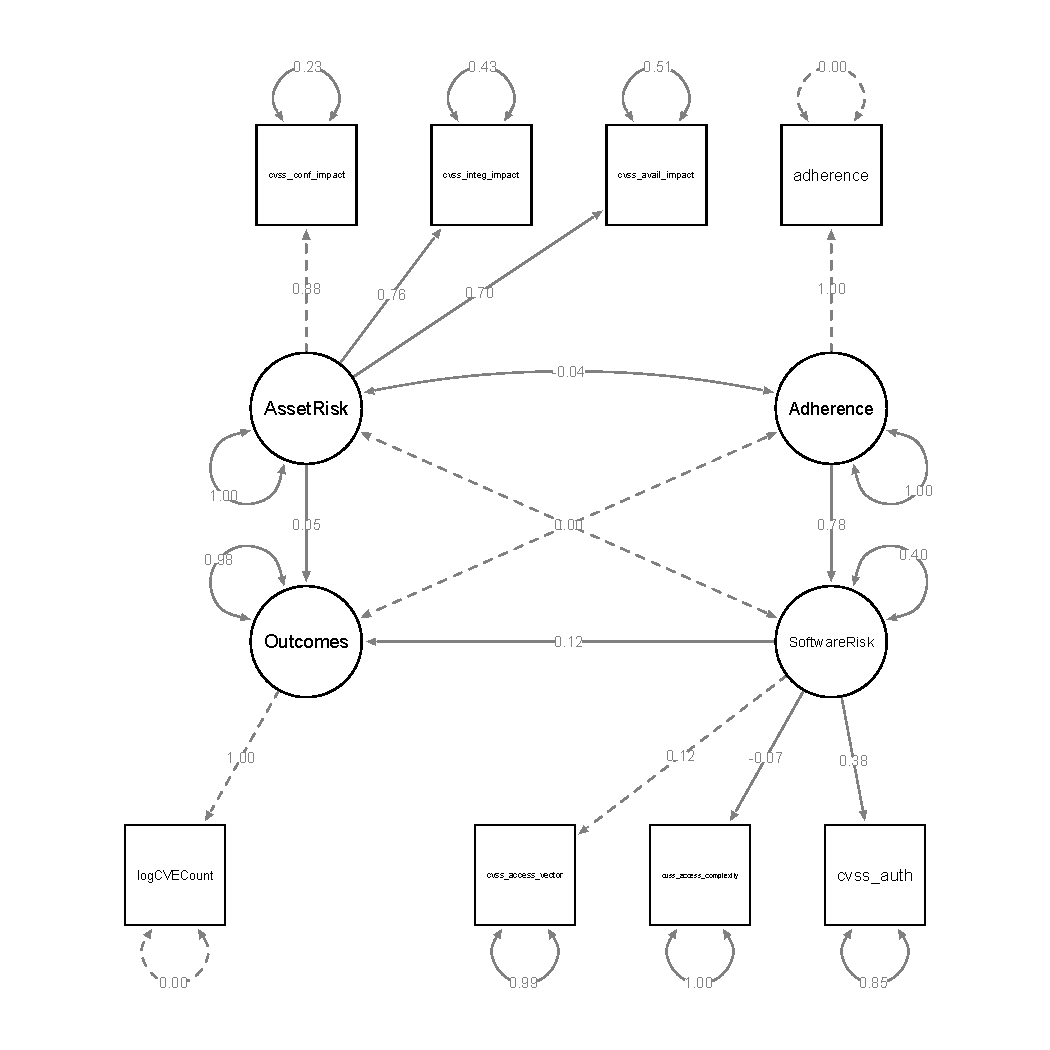
\includegraphics[width=.6\textwidth]{NVD_Respecified_SEM_Model.pdf}
	\caption{Respecified NVD Model}
	\label{fig:nvd_model_respecified_estimates}
\end{figure*}

Interpreting the (standardized) parameter estimates in terms of our hypothesized construct relationships, we have the following:
\begin{itemize}
	\item  Asset Impact is positively associated (0.05) with Security Outcomes, as hypothesized.
	\item Software Risk is positively associated (0.12) with Security Outcomes, as hypothesized. 
	\item Practice Adherence is positively associated (0.78) with Software Risk, contrary to what we hypothesized. 
\end{itemize}	
All three relationships were statistically significant. 

We plot how the three impact risk scores change over time in Figure \ref{fig:nvd_vulns_impact}, and the CVSS access risk scores in Figure \ref{fig:nvd_vulns_auth}. 	
		
\begin{figure}
	\centering
	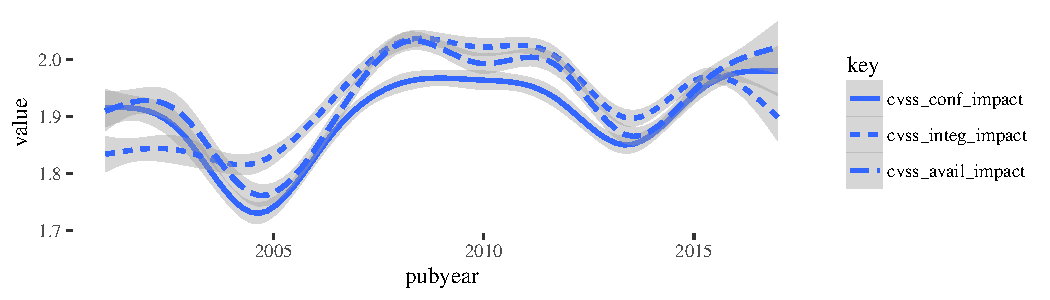
\includegraphics[width=\columnwidth]{nvd_cvss_impact}
	\caption{NVD CVSS Impact Risk by Year}
	\label{fig:nvd_vulns_impact}
\end{figure}

\begin{figure}
	\centering
	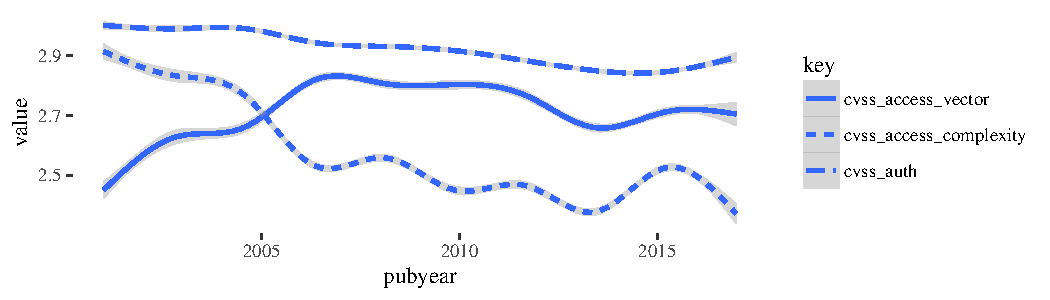
\includegraphics[width=\columnwidth]{nvd_cvss_auth}
	\caption{NVD CVSS Access Control Risk by Year}
	\label{fig:nvd_vulns_auth}
\end{figure}
\subsubsection{Discussion}
\label{sec:case_nvd_discussion}
In our data, Adherence has a strong effect on Software Risk (0.78 standardized). Translated to the measurements we used, more recent years are associated with higher Software Risk, Access Vector Risk has been increasing (CVSS access vector metrics have been deteriorating) over the last 15 years, and Authentication Risk has been decreasing (CVSS authentication metrics have been improving). The increase in web usage over the last 15 years correlates with the increase in network attacks represented by the access vector metric increase. However, the higher effort required by attackers over time is perhaps a positive reflection on the efforts of development teams to secure their software.  
 
We found effects for both Asset Impact and Software Risk on Security Outcomes, with Software Risk having an effect (.12 standardized) roughly two and a half times that of Asset Impact (0.05). We expect that at least one reason for the small (less than 15\%) effects of Asset Impact and Software Risk are due to the underlying measurement variables being incomplete accounts of the constructs they measure. For example, the impact metrics say something about potential risks, but do not say anything about the environments in which the software runs, or about the kind of data maintained by the software in the contexts from which vulnerabilities were reported. Similarly, the software risk constructs represented by CVSS access vector, and Authentication do not contain information on software size, churn, language, or the other constructs that have been identified as contributing to security issues in software. 

Asset Impact is correlated most strongly by the Confidentiality Impact measurement (.88 standardized), however the Integrity Impact (.76) and Availability Impact (.70) are in the same range and direction. Software Risk is correlated most strongly by Authentication Risk (0.38). Higher Authentication Risk, meaning lower number of authentications required by attackers, may imply that insufficient access control remains a significant development concern, although further investigation is warranted. Given the single measurements, we have no information on the relative importance of the measurements for Adherence and Outcomes constructs.

In general, the (standardized) residual variance values are higher than the .35 guideline established in Kline~\cite{kline2015principles}. The impact metric components of Asset Impact tend to have lower residuals as a group, suggesting that the three impact metrics may be reasonably explained in terms of a common construct. The Access metrics have high residuals, suggesting that the Access metrics may not be reasonably explained in terms of a common construct. 

We have to explain the unexpected negative association of Access Complexity Risk with Software Risk. One possible explanation is that Access Complexity is a poor measurement. The maintainers of the CVSS standard have acknowledged the overloaded nature of Access Complexity, stating that when it is applied it is impossible to tell if it is being used for user interaction from social engineering, from a race condition, uncommon configuration, attacker starting privileges, or anything else~\footnote{https://www.first.org/cvss}. However, each of the listed causes could be construed to be what we seek to measure for Software Risk. Version 3 of the CVSS (CVSSv3) scoring system includes a separate `User Interaction' metric to disambiguate between user-driven and software-driven reasons. In future work, we can update the measurement model to account for the updated CVSSv3 metrics. A second possible explanation is that measurement model is incorrect, via the Access Complexity metric being associated with the wrong construct, or a broader problem with assignments of metrics to constructs. To test this notion, we fit the model with Access Complexity associated with Asset Impact rather than Software Risk, but model fit was worse than when Access Complexity was associated with Software Risk. A third explanation is that our structural model is incorrect, either in the relationships between the constructs, or in missing one or more constructs with which Access Complexity could be associated. We put altering the structural model out of scope for the present work, but could investigate refinements of the structural model in future work. 

Per the descriptions of the metrics in Section \ref{sec:evaluation_nvd_selection_risk}, we view each of the metrics as measuring a property of the software that the development team can influence. Access Complexity Risk and Authentication Risk might be change through the addition, or refinement, of access control mechanisms. Alternatively, they might be increased by attacker discovery of alternate access paths.   Access Vector Risk might be reduced through care taken with validation of network inputs, or through greater care taken with implementation of network code, or increased through attacker path discovery. Authentication Risk might be reduced through stricter access controls, as with Access Complexity Risk, however the variables are not collinear in our data (as measured by Pearson's , Variance Inflation Factor). Authentication Risk might be increased, again by attacker discovery of alternative paths. Changes over time in each of the Access metrics may be due to development team efforts, or to attacker efforts, and we do not have the data here to distinguish between the two cases. We have assumed, in our modeling, that development team effort is the primary component for each metric. If attacker effort were the primary component, the metric should be modeled as part of Asset Impact.  If the three metrics we have were affected by different proportions of development team and attacker effort.

Our overall model data did not confirm Kaminsky's hypothesis that software quality is improving over time, with our adherence-over-time measure increasing Software Risk. However, we observed several counter-trends in the underlying data. We observed an improvement in CVSS Authentication Risk (Figure \ref{fig:nvd_vulns_auth}). On average, vulnerabilities are requiring more authentications over time, implying that development teams are putting an increasing amount of functionality behind access control.

We also observe from Figure \ref{fig:nvd_vulns_auth} that Access Complexity Risk has trended downward over time, in opposition to Authentication Risk and Access Vector Risk (Regressing Access Complexity Risk on adherence, controlling for the remaining measurement variables has a slope of -.09 for adherence, p-value \textless 0.001). The trend suggests that, on average, over time, vulnerabilities are becoming more complicated for attackers, likely for a variety of causes, but potentially implying that access control is being implemented more frequently over time by development teams.

On the other hand, CVSS Access Vector Risk has increased in parallel to the decrease in Authentication Risk, indicating that vulnerabilities are increasingly prone to remote attacks from across the network.